\documentclass[10pt,a4paper]{article}
\usepackage[utf8]{inputenc}
\usepackage{amsmath}
\usepackage{amsfonts}
\usepackage{amssymb}
\usepackage{listings}
\usepackage{graphicx}
\author{Richard Torenvliet - 6138861}
\title{Flood Simulation Browser}
\begin{document}
\maketitle
\section{Introduction}
This project concerns the Flood Simulation Browser. The concept of this browser is to illustrate/visualize a flood in a particular area. With this technology people can see the flow that the water will take. When a dike breaks it is important to know where the water will flow and at which time-step. Information about which locations in the area will be under water first can result in a successful evacuation plan. This system already exists but this project involves taking advantage of this system and make it easier available and accessible. Which makes it more likely that someone with the right authority can take decisions about placing dikes and creating a successful early warning system.
The implementation of this application will be on a multi-touch device. In particular iPad and Android tablets. Users can use this application in an intuitive way and get more intelligence about the complex situation at hand. They have the ability to choose from several simulations that where already made for a specific area and also creating new ones.
This document covers design choices/options in order to reach that goal. The first step is to get an idea of the existing simulation system of which this application will take use of. This includes a clarification of which part of the system this Browser will take. The next step will be finding what out the requirements of the tablet implementation, like what features does it have to contain in order to be to maintain the intuitiveness. Just by showing the data would not be sufficient. The function of this App is to extend the simulation system with a use-ability factor.
A side assignment of this project is testing the scalability of the REST server. By testing how much requests the server can handle at ones it helps the urban flood project to estimate how much people can use the application at ones. The original multi touch application on the multi touch table was only only one client. It's important to know that an early warning system stays online under the pressure of al lot of clients.

\section{Flood Simulation System}
The system that already exists runs in the Cloud. That means it does all the calculation for the client and it is not important to know at which physical computer it runs. The system can calculate other simulation by providing parameters about a certain area. When a simulation is run it will be stored in the system. With other calls the system returns a set of simulation that are present in the current database. Now the important thing to note is that the simulation consists of images that have to be displayed on a map, let's say Google Maps. The flood simulation system preforms a complex simulation with the height map of the area. The height map consists of detailed information about the height of an area. With this data the flow of the water can be calculated and turned in to images.
 
\subsection{Flood API}
The API is a REST api that returns a JSON formatted string. It's a client server system where requests are done by the client and the appropriate data is transferred back to the client. With this data, information about a certain simulation can be displayed. 


\subsection{Scalability}
A side assignment of the project is to test the scalability of the server. The server address is sangkil.science.uva.nl. To test this server it is needed to exclude any other parameter of the client. Such as maximum download speed, maximum throughput, latency of the network that the testing is finding place. The idea is not to test this at a home pc, but test it in a server that is hooked up in the same network as sangkil.science.uva.nl. If this is the case the exclusion of restricted variables at client side is possible. 
For stress testing the server there is a tool available called siege\footnote{http://www.joedog.org/siege-home/}. With this tool it is possible to launch request to a url with n-nodes with k fire-ing connections per second. Siege registers the following data:
\begin{itemize}
\item Transmissions - total
\item Elapsed Time - seconds
\item Data Transfer - (MB/s)
\item Response Time - 
\item Transfer Rate
\item Throughput
\item Concurrent
\item OKAY,
\item Failed
\end{itemize}
With this data new insight can be provided. By increasing the number of simultaneous connections, values could start to change. The expectations are that the response time might be longer. With more clients to serve, it could take longer if there are more clients active. If processor power is limited, maximum available memory is reached or the implementation of the server for handling requests could effect in the response time. 

\section{Flood Simulation App}
\subsection{Platform considerations}
As stated in the introduction the app is meant for tablets, but not specific for iOS or Android. How can we maintain this demand on the application? Is one of the research question. This means that the application is not native programmed but consists of one code-base and runs on more devices. There is a technology called PhoneGap that uses HTML5 CSS and Javascript to build the app. In essence the developer builds a mobile website and PhoneGap can wrap this in an application. The native web engine is that used to render the mobile website. PhoneGap can result in a huge speed-up in development which is a huge advantage because of the skills gained by webdevelopment can be re-used. Therefore there is no need to learn a new programming environment used for native apps in Objective C with Xcode for iOS and Java with Eclipse for Android. The advantage that is easy to learn and re-using earlier experiences in web development can be re-used, the disadvantage can be that it feels like a mobile website in stead of a native application. Luckily frameworks exists where native-like elements are created for you. 

This can be a Titanium Mobile, the Appcelerator. Titanium Mobile can build mobile applications that are in fact native applications. By programming in Javascript and call functions to create native elements. The framework builds native code, in contrary to previously discussed PhoneGap. The development for this platform is fast and an application for both iOS and Android are quickly of the ground. But there is also a disadvantage by using Titanium. The applications are big, around 11MB no matter what. Not only is do they take a lot of space on the storage device, but also has trouble of memory leaks(link).  Developing and testing on iOS provides expected behaviour and a lot is possible, for Android the native elements are mostly not the elements you thought the look like. To reach cross-platform apps you need to constantly check if your building an element for iOS or for Android. It might be stated that the functionalities of the platforms are randomly picked from the API. The idea of Titanium Mobile is great, it works fine but will delay developing time when you truly want to reach crossplatform. 

\subsubsection*{Javascipt frameworks}
As already explained, PhoneGap only provides the possibility to create an app out of a website. This website can be build in any way the developer likes using webtechnologies supported on the native device. There are frameworks that can speed up the development to make an intuitive application. Two frameworks that can be considered jQuery Mobile and Sencha Touch. 
\begin{description}
\item [jQuery Mobile]
This Javascript framework is build out of one Javascript file and one css file that the developer includes. By giving certain HTML elements a data attribute, which is a HTML5 element, the framework uses this to create views. A page is made by declaring a div adding data-role="page". Such a page can be given a footer like div data-role="footer". 
Switching frame one page to the other can be as simple as giving a html anchor a href to an id of a page. The next example will result in two pages, the both pages have a button. Both buttons link to the other page (foo, bar), so tapping on one button will change the page to the other page.
\begin{figure}
\begin{lstlisting}
<div data-role="page" id='bar'>
	<a #href='foo' data-role="button">switch to foo</a>
</div>

<div data-role='page' id='foo'>
	<a #href='bar' data-role="button">switch to bar</a>
</div>
\end{lstlisting}
\caption{jQuery Mobile, pages example}
\end{figure}

Creating to pages are quickly made, the downside of jQuery mobile is that in order to create an application where views look a like, you have to repeat yourself. You have to create pages with other id's but with the same  The conclusion is that jQuery mobile is really easy and the developer does indeed use html, css to create views.  But it is not easy to build a modular application. It is always possible to create such a modular application yourself, but when creating an application which is not such a framework the developer will run in to creating a framework in stead of the intended application.

\item [Sencha Touch 2]
Sencha touch 2 is a framework focused on the Model View Controller design pattern. It encourages the developer to use this pattern. The way of developing really differs from jQuery mobile. There where jQuery mobile sets you free to do whatever you like, sencha touch constraints the developer using components that are available in sencha touch. The difference can be easily explained with an example.

\begin{figure}[h!]
\begin{lstlisting}
Ext.application({
    name: 'foo',

    launch: function() {
        Ext.create("Ext.tab.Panel", {
            fullscreen: true,
            items: [
                {
                    title: 'bar',
                    iconCls: 'bar',
                    html: 'bar'
                }
            ]
        });
    }
});
\end{lstlisting}
\label{fig:sencha}
\caption{Sencha Touch application example}
This example creates an application with the name 'foo'.  The html can be placed inside the items array. 
\end{figure}
\end{description}
In the items array in the example there but other items like lists, tabview or a map. And items are configured with the config attribute. Any component present in the sencha touch framework. The advantage is an application that is structured out of the box with a design pattern that is current standard(MVC). With sencha touch 2 there is no need for PhoneGap, unlike jQuery Mobile. Sencha Touch 2 provides the possibility to run the code on your simulator or native device by the command line tool. Testing for Android an iOS became much more simplistic resulting in less developing time. Running PhoneGap for Android needs Eclipse to build, on iOS you need to build in the Xcode. When testing on both devices you'll need to be able to test in both environments which is highly less desirable than building from command line. A disadvantage of sencha touch could be, as seen in figure \ref{fig:sencha}, the syntax of sencha touch is not so easy at first. So the learing curve could be very .

\subsection{App Design}
The application will be used on tablets so a lot of space can be used. Working with tablets the screen gets larger than mobile phones. Which can result in a bigger travel distance of the user's hands. The GUI design has to be build with the considerations of the interaction capability of the users. For instance, unlike with mobile phones, according to Clark(2012) a leading designer in creating multi-touch applications, people intend to hold a tablet on the top halve of the tablet when holding with both hands, figure \ref{fig:perimeter}. The focus of the user is going from top to down. The top elements of the application will draw the first attention of the user. That's why Clark(2012) advises to place the important controls on the top half of the screen. The components that are important have to be placed in the left or right top of the screen. By taking Clark's advise the Flood Simulation Browser can be inspired. 
First of all the flood simulations are within different cities. This can typically be a list of cities, also a list is scrollable and can be seen as an infinite array of cities around the world. Every city has it's own array of simulations to show. So it makes sense to also show these in a second list. When a city is selected, the user has no use of the capability to select other cities and it's simulations. This is because it makes sense to only have one Map object in the view where one location (latitude, longitude) can be shown at a time. The map object is the component that is the important part of the browser. Inspired by Clark(2012) it can be stated that a hierarchy in importance of different view components can result in a different place on the screen. By placing the Map component always in the view and also as the biggest component the idea of placing objects in a hierarchy of importance in the view is considered.
The list component where cities and simulations are placed is the left side of the view, it could also be the right side but it would not matter. Two hands are more or less symmetrical so placing the list object left or right would not be a problem. It does matter concerning controls, but which controls shown in the top bar is not clear at this moment. Controls that would be needed is the ability to change the image placed on the map. A simulation consists of multiple images on different time steps. By giving the user control of which image is seen at which time step is a crucial feature in the browser. 
The flood simulation browser already build for the multi touch table has the ability to submit new simulations to be simulated in the cloud. The spot of the simulation can be arbitrary on the map, by simply touching a place on the map and alter some parameters the cloud service can create a new simulation to be seen. Although this feature can be an seen as an extension of my project with time left, this feature can be build in. That's why it can be considered in the App's design. The controls of these parameters need to be somewhere in view, by placing this in the neighbourhood of the place where the user placed touched the map could be intuitive. But not if happens when your only are browsing through the map, the user has to know that it is in the mode of with picking a place where to create a new simulation. The specification about these controls are discussed in the end report.


\begin{figure}[h!]
\center
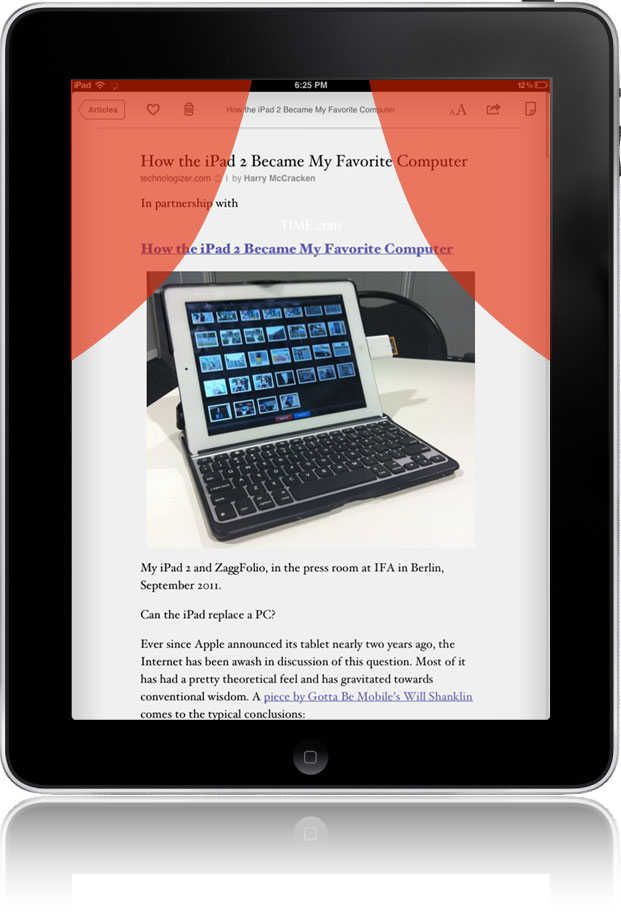
\includegraphics[scale=0.3]{touch.png}
\caption{Portrait touch perimeter(Clark, 2012)}
\label{fig:perimeter}
\end{figure}


%http://www.netmagazine.com/features/designing-touch  John Clark 2012 on February 01, 2012 
\end{document}